%\ifthenelse{\boolean{arxiv}}{
\begin{figure*}[t]
    \centering
    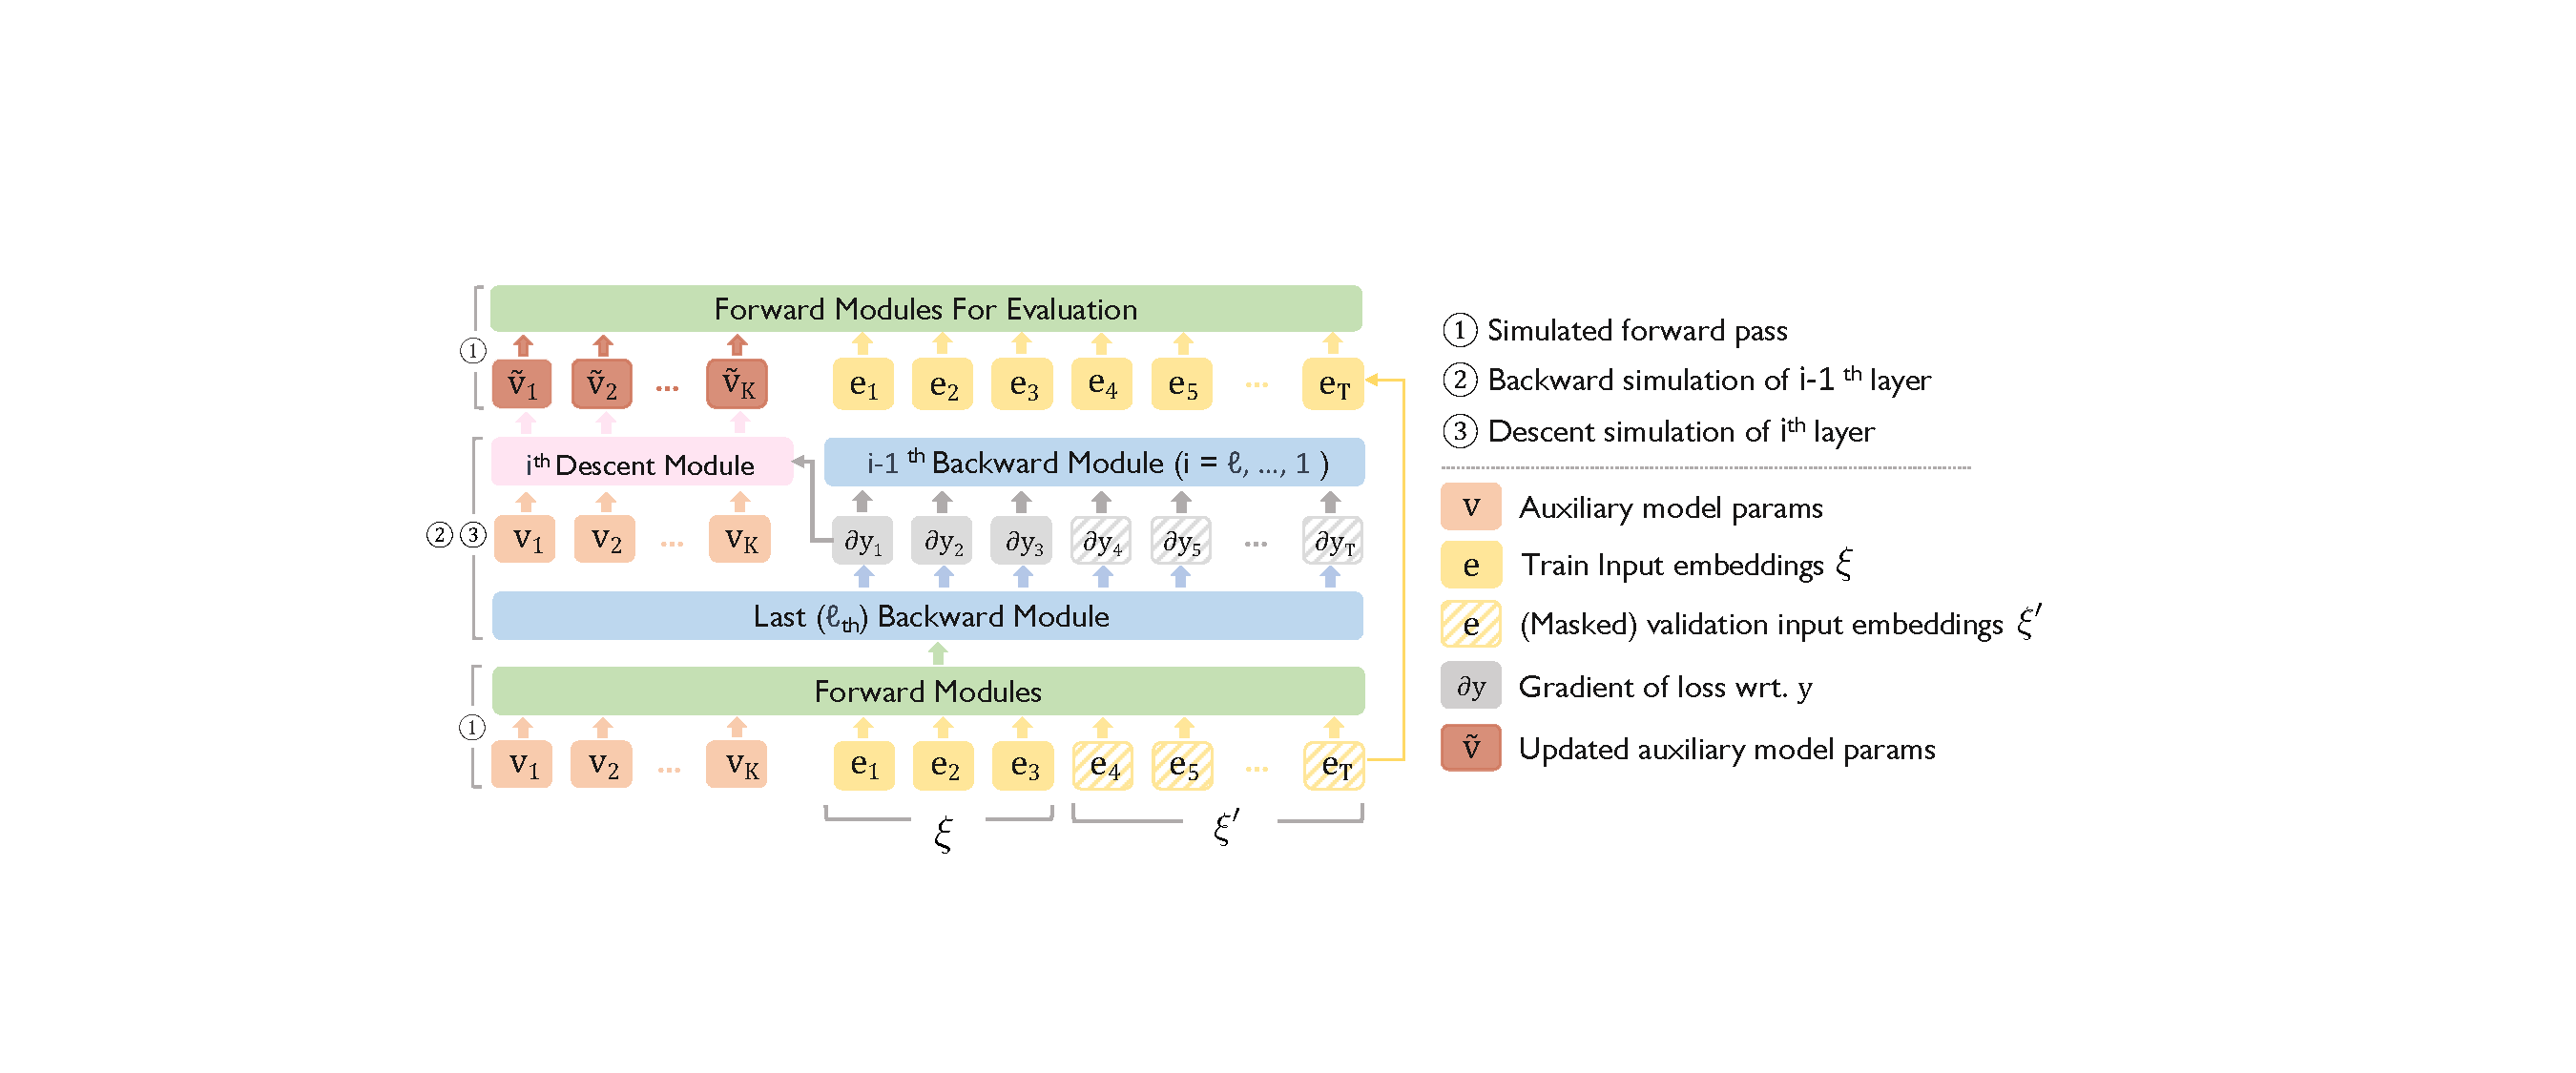
\includegraphics[width=\textwidth]{figures/Final_images.pdf}
    \caption{The overall structure of \textsc{TinT} (see~\Cref{sec:design} for an overview). Each forward, backward, and descent module is represented using combinations of linear, self-attention, layernorm, and activation layers.
    The input consists of prefix embeddings (\Cref{def:prefix_embs}) that represent relevant auxiliary model parameters in each layer followed by natural language input. A prefix mask separates the train and test segments of the input (\textsection\ref{sec:input_structure}). 
    %Auxiliary model parameters are updated in the descent module using the training part, and the updated prefix tokens are transferred to the forward modules via residual connections for evaluating the rest. 
    %\snote{Update figure to contain $\xi$ and $\xi'$ notation.}
    }
    \label{fig:general_structure_simulator}
\end{figure*}
%}{

\iffalse
\begin{figure}
    \centering
    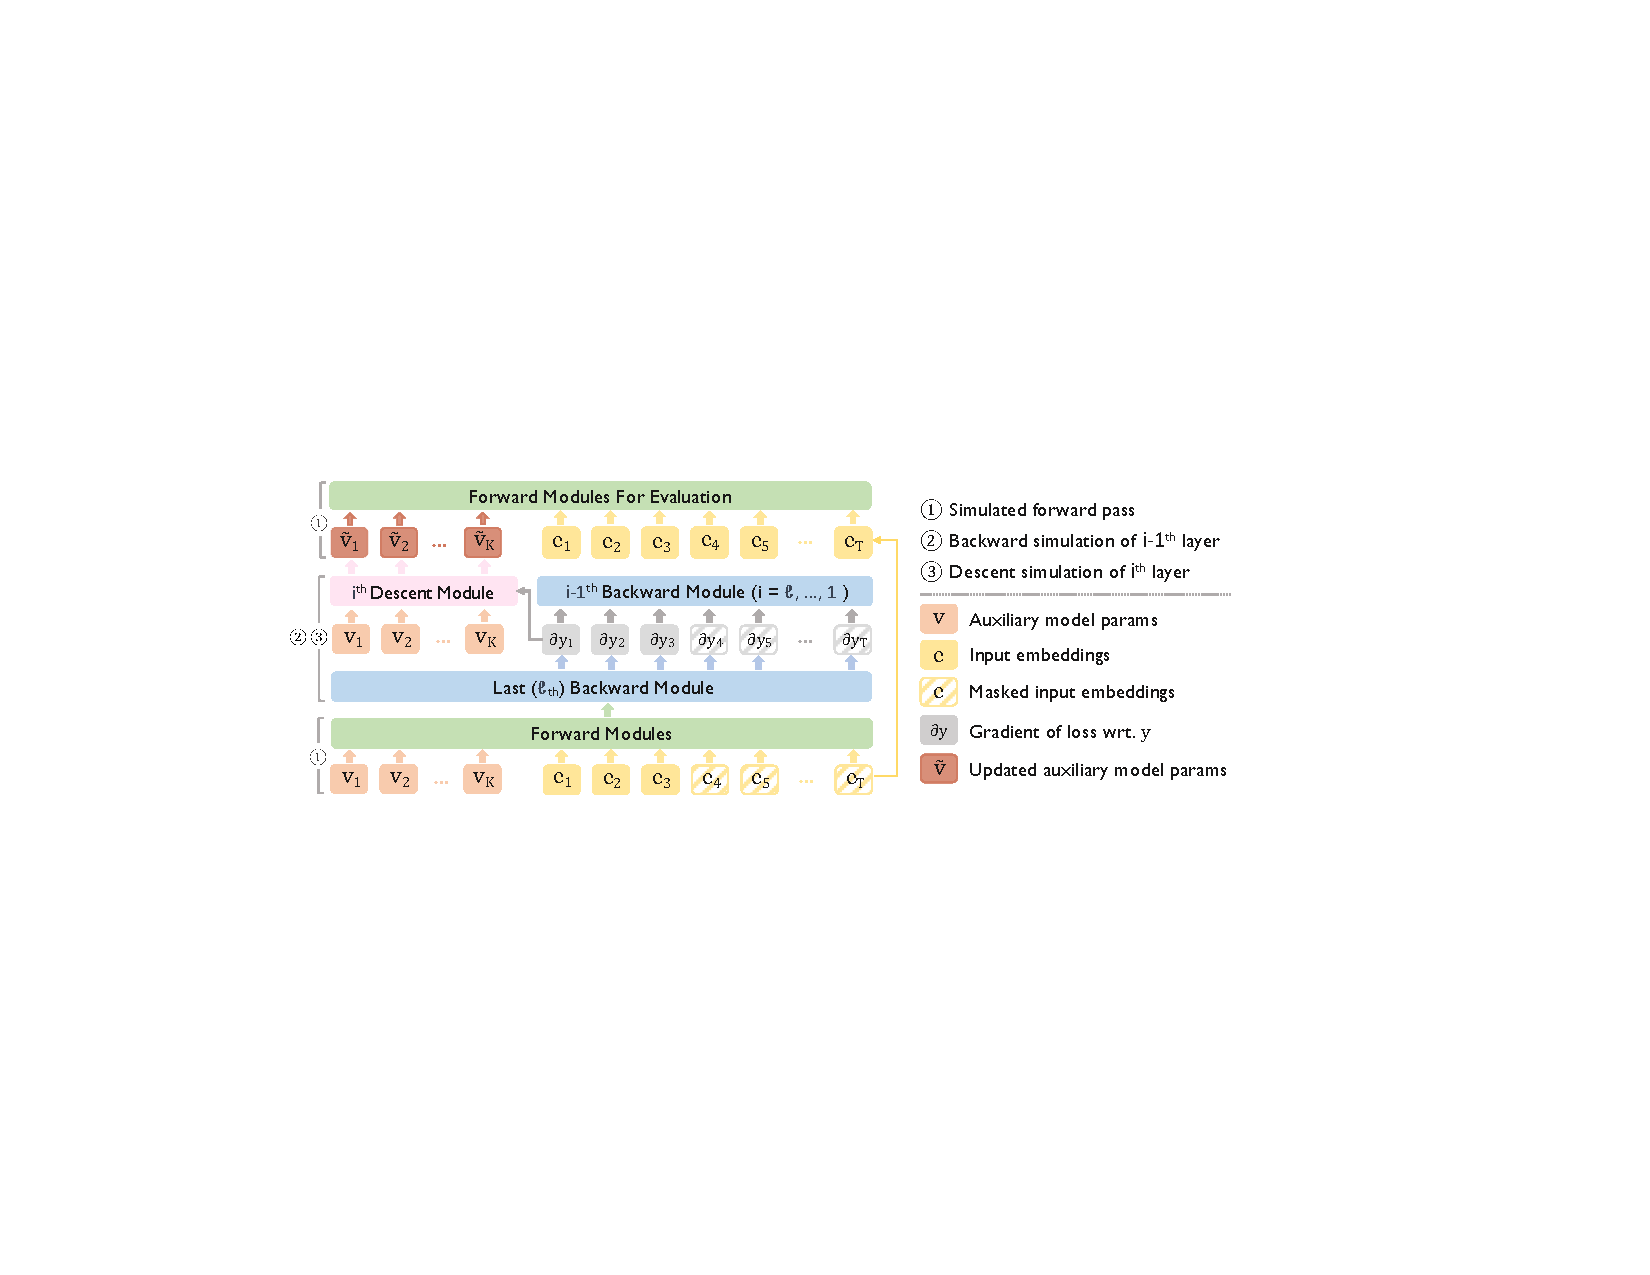
\includegraphics[width=\textwidth]{figures/figure1.pdf}
    \caption{The overall structure of \textsc{TinT}. The input consists of prefix embeddings, that represent relevant auxiliary model parameters in each layer, input token embeddings, and a binary prefix mask to separate the train and evaluation segments of the input. The auxiliary model parameters are updated in the descent module using the training part of the segment, and the updated prefix tokens are transferred to the forward modules via residual connections for evaluating the rest of the segment. 
    }
\end{figure}
}
\fi


\begin{figure*}[t]
    \centering
    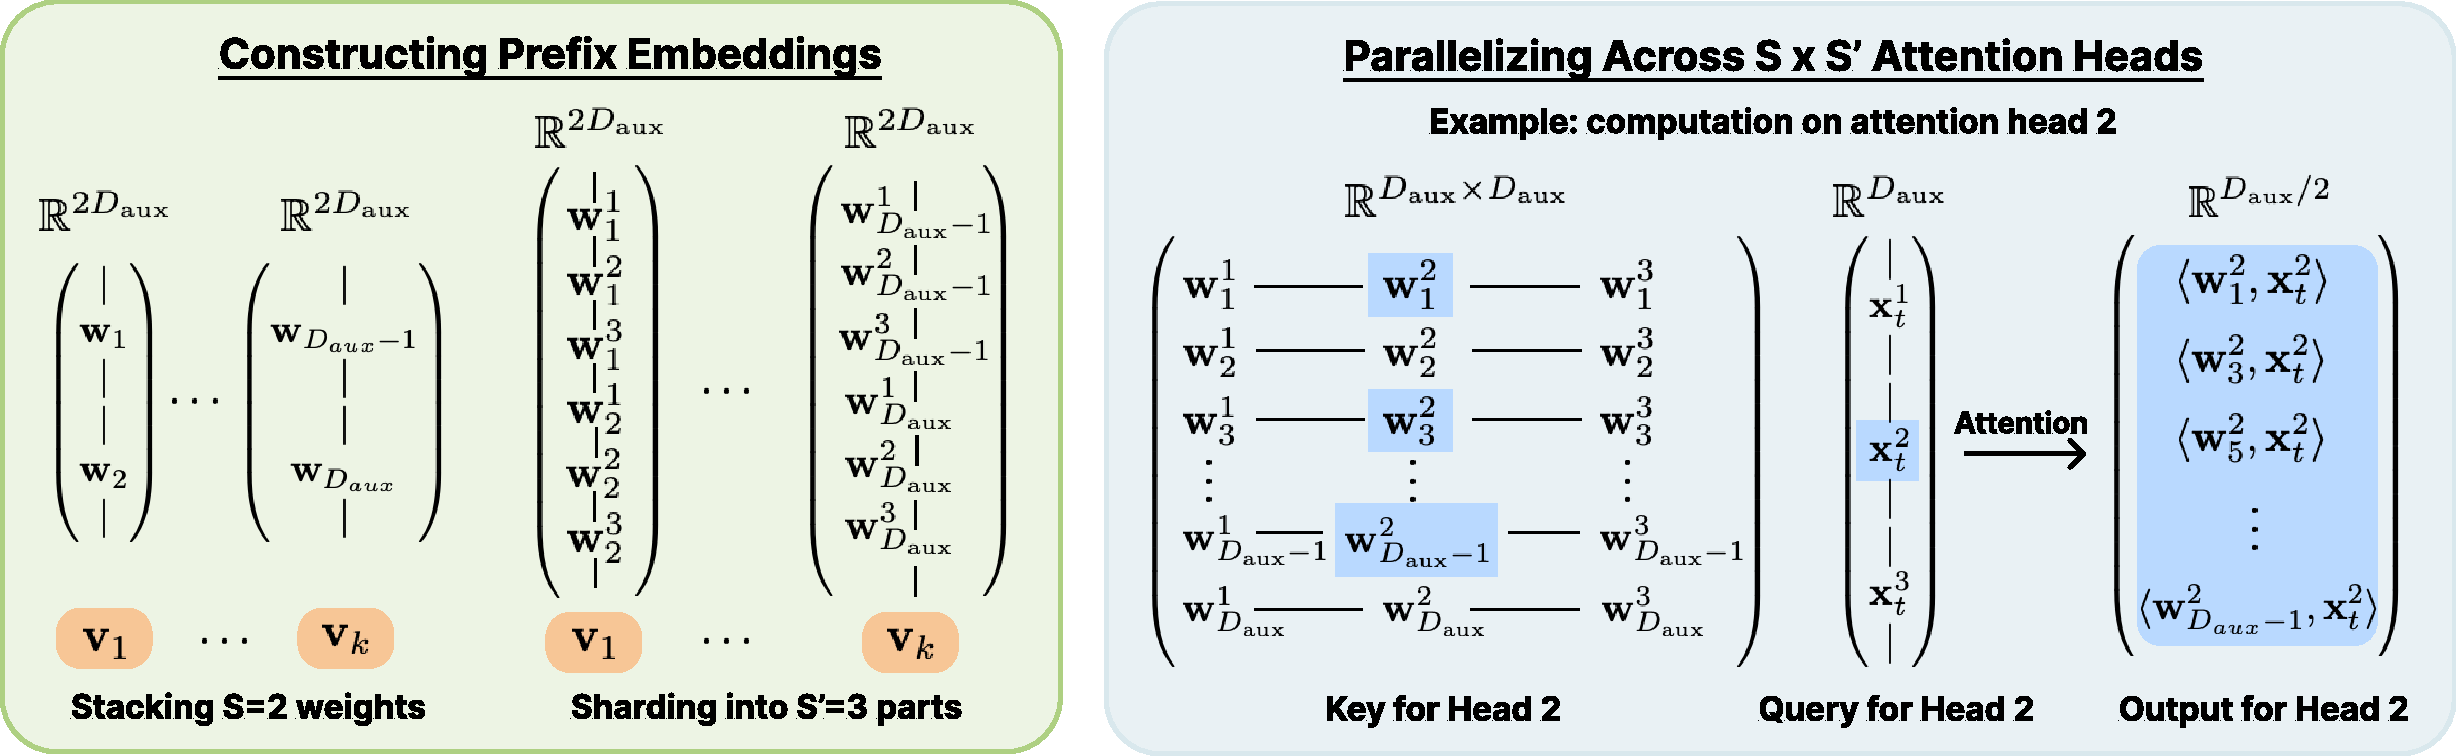
\includegraphics[width=\textwidth]{figures/linearforward_v3.pdf}
    \caption{\simulator{} simulates the forward pass of a linear layer with a $\simu{H}$-head attention layer ($\simu{H}=6$ here). We stack $S$ weights per prefix embedding to reduce the number of prefix embeddings required ($S=2$ here). We furthermore shard each weight and token embedding $\vx_t$ into $S'$ shards and compute inner products of each shared in parallel using $S \times S'$  attention heads ($S'=3$ here). Please see~\Cref{sec:stack}.}
    \label{fig:linear_forward}
\end{figure*}


\section{Design Considerations}\label{sec:design}
Our goal is to construct a simulator that can train an auxiliary model over the course of an inference pass. 
This procedure requires four steps:
\begin{enumerate}[leftmargin=*]
	\item \textbf{Forward Pass}: A forward pass to compute the auxiliary model output $f(\xi;\aux{\vtheta})$ on training input $\xi$ and a loss $\Loss$.
	\item \textbf{Backward Pass}: Backpropagation to compute the gradient of the auxiliary model $\nabla_{\aux{\vtheta}} \Loss(f(\xi;\aux{\vtheta}))$.
	\item \textbf{Parameter Update}: Update the auxiliary model using gradient descent, setting $\aux{\vtheta}' = \aux{\vtheta} -\eta\nabla_{\aux{\vtheta}} \Loss(f(\xi;\aux{\vtheta}))$.
	\item \textbf{Output}: Output next-token predictions $f(\xi';\aux{\vtheta}')$ on a test input $\xi'$ using the updated auxiliary model. %Output these predictions as the simulator output.
\end{enumerate}
Note that steps 1-3 can be looped to train the auxiliary model for a few steps\footnote{Looping steps 1-3 scales the depth of the simulator model.}, either on the same training data or on different training data for each step, before evaluating it on the test input~\citep{giannou2023looped}. 
The above method highlight two crucial features of the simulator: (1) it has access to some amount of training data, and (2) it can use (i.e., read) and update (i.e., write) the auxiliary model.
Below, we discuss how to design a modest-sized simulator around these two considerations.

\subsection{Input structure}\label{sec:input_structure}
For simplicity, we describe only one update step on a single batch of training data $\xi$ but note that our formal construction and our experiments handle multiple training steps (see~\Cref{def:finetune}).
Steps 1 and 4 show that the simulator must access some training data $\xi$ to train the auxiliary model and some testing data $\xi'$ on which it evaluates the updated auxiliary model. 
For the sake of illustration we consider the following simple setting: given a sequence of input tokens $\ve_1,...,\ve_T$, we split it into training data $\xi=\ve_1,...,\ve_r$ and testing data $\xi'=\ve_{r+1},...,\ve_T$.

Suppose $\xi$ contains an in-context input-output exemplar and $\xi'$ contains a test input.
Then, the simulator performs a very natural operation of training the auxiliary model on a task-specific example and outputs results for the test example. 

On the other hand, if the input is not specially formatted, $\xi$ and $\xi'$ may simply contain some natural language tokens.
In this case, the simulator is using the first part of the context tokens to do a quick fine-tune of the auxiliary for some task before outputting the subsequent tokens with the auxiliary model. In a worst-case scenario, users might provide harmful contents, leading the model to implicitly fine-tune on them and potentially output even more harmful content. 


Our experiments consider many options for splitting a sequence into $\xi$ and $\xi'$, and we defer a more detailed discussion of possible setups to~\Cref{sec:experiments}.

\looseness-1\paragraph{Accessing Training Labels.} 
The simulator must be able to see the labels of the training tokens 
in order to compute the loss $\cL$ (usually, the autoregressive cross-entropy loss) in step 1. 
For example, in \cref{fig:general_structure_simulator}, when we compute the loss for the token $\ve_2$ in the second position, we need to use its label $\ve_3$ in the third position.
However, this is not possible if the simulator uses strictly autoregressive attention (\cref{sec:lm_head} contains a more general discussion).
We thus use a bidirectional attention mask on the training tokens and autoregressive attention on the evaluation portion.
We note that encoding relevant (e.g., retrieved) context with bidirectional attention is a popular way to improve autoregressive capabilities in language modeling and natural language tasks~\citep{raffel2020exploring,borgeaud2022improving,izacard2020leveraging,izacard2023atlas,wang2023shall,tay2022ul2}.
This empirical approach is similar in motivation to how \simulator{} uses a few context tokens to adapt the auxiliary model to a given input.
Having established the training and testing data, we can now move to discussing how the simulator can access (i.e., read) and update (i.e., write to) the auxiliary model at inference time.  

\subsection{Read and write access to auxiliary model}
As discussed in the start of this section, the simulator must have read and write access to the parameters of the auxiliary model.
Crucially, the simulator must do at least two forward passes through the auxiliary model, one with the current parameters $\aux{\vtheta}$ and one with the updated parameters $\aux{\vtheta}'$.

The straightforward  way to simulate the forward pass of the auxiliary model would be to store its weights in the simulator's weights and run a forward pass as usual.
One can analogously simulate the backward pass according to the loss $\Loss$ to compute the gradients.
However, \textbf{the simulator cannot update its own weights at inference time}, so this strategy would not permit the model to write the updated parameters $\aux{\vtheta}'$ and later read them when simulating the second forward pass.
Therefore, the auxiliary model $\aux{\vtheta}$ must be available in the activations of the simulator. 

To this end, \citet{wei2022statistically,perez2021attention} model the simulator after a Turing machine, where the activation $\ve_t^{(\ell)} \in\RR^{\simu{D}}$ in each layer acts as a workspace for operations, and computation results are copied to and from memory using attention operations.
In this paradigm, if $\aux{D} = 768$, computing a dot product $\langle \vw, \vx_t^{(\ell)}\rangle$ with weight $\vw\in\RR^{768}$ requires at least $6.4$ million parameters in the simulator\footnote{
Using a feedforward module to mimic the dot product (as in \citet{akyurek2022learning}, see thm. \ref{thm:gelu_multiplication}), where the simulator embedding comprises $[\vw, \vx_t] \in \RR^{1536}$, necessitates a minimum of $4.7$ million parameters. Using an attention module to copy the weight from memory adds another $1.7$ million parameters.}.
Given the pervasiveness of dot products in neural network modules, this strategy would yield a simulator with trillions of parameters. 


Alternatively, one can store parameters in the first few context tokens and allow the attention modules to attend to those tokens~\citep{giannou2023looped}. 
This removes the need for copying and token-wise operations. 
Then, the same dot product requires only a self-attention module with $1.7$ million parameters.
We thus adopt this strategy to provide relevant auxiliary model weights as \emph{prefix embeddings}.
\begin{definition}[Prefix Embeddings]
    $\{ \vv_j^{(\ell)} \}_{j=1}^K$ denotes the $K$ prefix embeddings at the $\ell$th layer  in \simulator . These contain \emph{relevant} auxiliary model weights or simulated activations.
    \label{def:prefix_embs}
\end{definition}
We now consider how to efficiently simulate the building block of neural networks: matrix-vector multiplication.
In the next section, we demonstrate that a careful construction of the prefix embeddings enables efficient parallelizaton of matrix-vector products across attention heads.


\section{Efficient Forward Propagation}\label{sec:exposition_linear_forward}
We now discuss how \simulator{} performs a highly efficient forward pass through the auxiliary model.
Here, we focus on the linear layer  because it is repeated many times in various transformer modules (e.g., in self-attention), so improving the efficiency dramatically reduces \simulator{}'s size.
\begin{definition}[Linear layer]\label{def:linear_mainpaper}
    For a weight $\mW\in\RR^{\aux{D} \times \aux{D}}$, a linear layer takes $\vx\in\RR^{\aux{D}}$ as input and outputs $\vy = \mW\vx$.\footnote{Linear layers are applied token-wise, so we can consider a single position $t$ without loss of generality.}
\end{definition}
We compute $\vy$ coordinate-wise, i.e., $\langle \vw_i, \vx_t\rangle$ for all $i \in [\aux{D}]$, where $\vw_i$ is the $i$th row of $\mW$. 
The simulator represents $\langle \vw_i, \vx_t\rangle$ as an attention score between the row $\vw_i$ and the input $\vx_t$. 
So, the input embeddings $\ve_t$ contain $\vx_t$ in the first $\aux{D}$ coordinates, and the rows $\{\vw_i\}$ of the weight matrix $\mW$ are in prefix embeddings $\{\vv_j\}$ (def. \ref{def:prefix_embs}).

We strategically distribute the weights (\textsection\ref{sec:stack}) and aggregate the parallelized computation results (\textsection\ref{sec:aggregate}).
As we briefly mentioned in the previous section, a straightforward construction of the linear layer would use the context and attention heads inefficiently.
Our construction instead parallelizes the computation across attention heads in such a way that aggregating the output of the linear operation can also be conducted efficiently.



\subsection{Stacking and Sharding}\label{sec:stack}
We partition the inner product computation across attention heads by carefully rearranging the weights and activations via stacking and sharding (\Cref{fig:linear_forward}).

Instead of representing each weight $\vw_i$ as its own prefix token $\vv_i$, we \emph{stack} $S$ weights on top of each other to form each prefix embedding $\vv_i$. $S$ drives a trade-off between the embedding dimension of the \simulator, $\simu{D}= \aux{D}S$, and the context length to the \simulator, $\simu{T} = K+\aux{T}$. 
We set $S=4$.


A simple strategy now would be to use different attention heads to operate on different rows; however, this would still use only $S$ attention heads whereas we could parallelize across many more heads.
We instead parallelize across more attention heads, where each head is responsible for computing the inner product on a subset of the coordinates. % while ensure the resulting output can easily be compiled:
We \emph{shard} each individual weight and the activation into $S'$ parts and compute the inner product on each of the $S'$ parts in parallel 
We set $S$ and $S'$ such that $\simu{H} = S\times S'$, thereby using all of \simulator{} heads to efficiently compute the dot products. 

\subsection{Efficient Aggregation}\label{sec:aggregate}
The attention module outputs a sparse matrix with shape $(\simu{D} / \simu{H})\times \simu{H}$ containing the inner products on various subsets of the coordinates in its entries.
To complete the linear forward pass, we need to sum the appropriate terms to form a $\simu{D}$-length vector with $\mW\vx$ in the first $\aux{D}$ coordinates.
Straightforwardly summing along an axis aggregates incorrect terms, since the model was sharded.
On the other hand, rearranging the matrix would require an additional $\simu{D}\times\simu{D}$ linear layer.
Instead, \simulator{} saves a factor of $\simu{H}\times$ parameters %\mz{anything missing here?} 
by leveraging the local structure of the attention output.
We illustrate this visually in \cref{sec:H-split_operation_app}.
This procedure requires $\simu{D}^2/\simu{H} + \simu{D}\simu{H}$ parameters. 
This efficient aggregation also compresses the constructions for the \simulator's backpropagation modules for layer normalization and activations (\cref{sec:LNappendix,sec:act_appendix}).


